\documentclass{report}
\usepackage{setspace}
\usepackage{bookmark}
%\usepackage{subfigure}

% my extra package imports;
\usepackage{caption}
\usepackage{algpseudocode}
\usepackage{algorithm}
\usepackage{float}
\usepackage{hyperref}
\usepackage{subcaption}
\usepackage{graphicx}
\usepackage{graphics}
\usepackage{tikz}
\usetikzlibrary {positioning, shapes, bayesnet}
\graphicspath{{./}}
\usepackage{natbib}
% end of my imports;

\pagestyle{plain}
\usepackage{amssymb,color}
\usepackage{amsfonts}
\usepackage{latexsym}
\usepackage{a4wide}
\usepackage{amsmath}

\newtheorem{theorem}{THEOREM}
\newtheorem{lemma}[theorem]{LEMMA}
\newtheorem{corollary}[theorem]{COROLLARY}
\newtheorem{proposition}[theorem]{PROPOSITION}
\newtheorem{remark}[theorem]{REMARK}
\newtheorem{definition}[theorem]{DEFINITION}
\newtheorem{fact}[theorem]{FACT}

\newtheorem{problem}[theorem]{PROBLEM}
\newtheorem{exercise}[theorem]{EXERCISE}
\def \set#1{\{#1\} }

\newenvironment{proof}{
PROOF:
\begin{quotation}}{
$\Box$ \end{quotation}}



\newcommand{\nats}{\mbox{\( \mathbb N \)}}
% \newcommand{\rat}{\mbox{\(\mathbb Q\)}}
\newcommand{\rats}{\mbox{\(\mathbb Q\)}}
\newcommand{\reals}{\mbox{\(\mathbb R\)}}
\newcommand{\ints}{\mbox{\(\mathbb Z\)}}

%%%%%%%%%%%%%%%%%%%%%%%%%%

% COVER PAGE;
\title{
  { \includegraphics[scale=.5]{ucl_logo.png}}\\
  {{\Huge Graph style transfer using Inverse Reinforcement Learning}}\\
  % {\large An application to subway networks}\\
}

\date{Submission date: 11 September 2023}
\author{
  Candidate Number: YLLK3\thanks{
      {\bf Disclaimer:}
      This report is submitted as part requirement 
      for the MSc Machine Learning at UCL. It is
      substantially the result of my own work except 
      where explicitly indicated in the text.
      The report may be freely copied and 
      distributed provided the source is explicitly acknowledged.
    }
    \\ \\
  MSc Machine Learning\\ \\
  Supervisors: Prof. Steve Hailes, Prof. Mirco Musolesi, Dr. Victor-Alexandru Darvariu
}

\numberwithin{equation}{section}
\numberwithin{figure}{section}
\numberwithin{table}{section}  
\numberwithin{algorithm}{section}

%%%%%%%%%%%%%%%%%%%%%%%%%%%%%%%%%%%%%%%%%%%%%%%%%%%%%%%%%%%%%%%%%%
% START DOCUMENT;
\begin{document}
\onehalfspacing
\maketitle

%%%%%%%%%%%%%%%%%%%%%%%%%%%%%%%%%%%%%%%%%%%%%%%%%%%%%%%%%%%%%%%%%%
% ABSTRACT;
\begin{abstract}
  \textbf{I THINK THIS IS DONE}


  In this report we investigate methods for learning a graph 
  construction mechanism based on a single graph example. We 
  tackle this problem from the angle of Inverse Reinforcement Learning 
  (IRL) whose goal is to learn a reward function given 
  expert demonstrations. 
  
  After learning a reward function, we use it as an 
  objective on a different graph and learn a 
  new policy to perform style-transfer.  
  The style-transfer constitutes transferring the topological 
  propoerties of the source graph to the target graph, while 
  preserving the vertex set attributes of the target graph.
  
  We investigate different ways to achieve this and 
  propose improvements over current methods with respect 
  to decreasing the variance during training of the IRL procedure. 
  These improvements are inspired by the 
  literature on per-decision importance samples 
  in Reinforcement Learning, exploiting conditional independence 
  properties of rewards given states and actions.
  
  In our experiments, we test two ways to achieve style-transfer 
  on graphs. First, we try  
  directly deploying the 
  jointly learned (together with the reward)  
  policy from IRL based on the source graph, 
  on the target graph. Second, 
  we train 
  a new policy on the target graph using the learned reward 
  function from IRL and then sample trajectories from it. 
  In all experiments, we use GraphOpt as our baseline. 
\end{abstract}
\tableofcontents
\setcounter{page}{1}

%%%%%%%%%%%%%%%%%%%%%%%%%%%%%%%%%%%%%%%%%%%%%%%%%%%%%%%%%%%%%%%%%%
% NEW CHAPTER - INTRODUCTION;
\chapter{Introduction and Related Work}\label{chap:intro}
\textbf{I THINK THIS IS DONE;}

As more and more graph data become available, researchers in 
areas such as biology \citep{VGAEDisease}, quantum chemistry 
\citep{MPNNs}, social networks \citep{SocialNets} and others 
seek ways to analyse these data in a way that extracts 
maximum information 
and requires the least amount of hand-designed features.

When it comes to automatic feature-selection, Deep Learning (DL)
is among the most successful paradigms spanning domains like 
text \citep{textCNN,RNNs,SentimentRNN,BERT}, 
vision \citep{alexnet}, and even graphs \citep{ScarselliGNN,VGAE,GCN,GAT}.

The ability of DL to extract predictive features, and generaly 
arrive at continuous embeddings of abstract data types, makes 
it a prominent component of current Deep Graph Learning techniques.

Although methods such as ``node2vec'' and ``DeepWalk'' 
\citep{node2vec,DeepWalk} have been 
proposed to automatically learn node features based on random 
walks over the graph (ignoring node features), 
it has been shown that Graph Neural Networks 
(GNN) \citep{ScarselliGNN,GCN} achieve superior performance in domains 
such as citation graphs \citep{VGAE} and Disease-gene link prediction 
(DGP) \citep{VGAEDisease}, among others. 
It has been postulated that this is because 
of the way GNNs utilise node features during the (neural) 
message passing procedure. Unsurprisingly, this has sparked interest 
in engineering different architectures for neural message passing 
\citep{GCN,MPNNs,GAT,GATv2}.

Outside of prediction, there exist other graph tasks that may be 
of interest such as graph construction. Having access to a 
graph-generative mechanism allows 
one to create synthetic data from a given distribution, which can 
be used for data augmentation, for example. 

Graph-style transfer, is another 
venue of interest, where given a generative mechanism for 
a source graph, one can apply the same on a target graph in order 
to induce structure similar to that of the source graph. The 
last mentioned task is somewhat similar to Neural Style Transfer (NST) 
\citep{NSTGatys} from the computer vision literature, where we 
have a ``content'' image and a ``style'' image. The goal in NST 
is to transfer artistic traits of the ``style'' image 
(e.g., color or style of painting) to the ``content'' image 
while preserving the entities seen in the ``content'' image. In 
the graph setting, we can think of the style as the topology, 
while the content are the nodes (or node features).  

While many prediction tasks, such as edge and/or node-attribute 
prediction \citep{GCN,VGAE,VGAEDisease,node2vec,DeepWalk}, 
have been successfully tackled, 
the area of graph construction has only recently gained popularity 
\citep{Darvariu,DeepMindGraphGen,GCNPolicyGraphGen,GraphRNN,GraphOpt,olivecrona2017molecular,Yang2017}.
Some methods 
utilise probabilistic formulations of the graph generative 
procedure \citep{NetGAN,DeepMindGraphGen,GraphRNN}, 
while others frame graph 
construction as a sequntial decision-making problem 
\cite{Darvariu,GraphOpt,GCNPolicyGraphGen,Yang2017,olivecrona2017molecular}. 
This work 
is concerned with the latter approach to graph generation. 

While \cite{Yang2017} and \cite{olivecrona2017molecular} 
still frame graph construction as a 
sequential decision making problem, 
they use simplified molecular-input line-entry system (SMILES) to 
encode molecules (the graph domain in their application). 
This is in contrast to the works of \citet{Darvariu,GCNPolicyGraphGen,GraphOpt},
where the graphs are the states and embeddings are obtained 
from a GNN 
encoder. The work of \citet{Darvariu,GCNPolicyGraphGen,GraphOpt} 
is therefore, more relevant to our application. 

In their application for generating edges in urban-networks, 
\cite{Darvariu}, exploit the knowledge of the dynamics of 
the MDP and use Monte Carlo Tree Search (MCTS), a discrete 
model-based control algorithm, to arrive at 
graphs which are optimised for 
Efficiency and Robustness. These are metrics that were assumed 
to be important for the construction of urban networks. Intuitively, 
high Efficiency implies that the graph is ``well-connected'' and 
information can flow via fewer edges from any given node to any 
other node. Robustness can be understood as the property of 
stability given a deletion of a node - ``how 
much does the deletion of one node impact the information flow 
of the network''. The mentioned work uses fully hand-designed 
rewards to specify the goal of the agent.

On the other hand, in their application to 
molecule construction, 
additionally to hand-designed properties, \cite{GCNPolicyGraphGen}
incorporate ``prior knowledge'' to the graph generation task, which 
they argue, constrains the generated molecules to resemble the 
molecules observed in a given dataset without harming the 
policy's ability to explore. This prior knowledge is 
summarised in the loss function of a Discriminator network trained 
jointly with a Generator on a given dataset. Similarly to \cite{Darvariu}, 
graph embeddings are obtained using a GNN encoder taking a graph 
object as input. This is argued to additionally stabilise the 
performance of the algorithm, as opposed to using 
simplified molecular-input line-entry system (SMILES) as 
graph embeddings.
 The RL part is achieved by policy gradients 
on the given hand-engineered 
reward signals combined with the loss of the Discriminator 
network. Furthermore, \cite{GCNPolicyGraphGen} promote the RL 
approach to graph generation due to the fact that it can explore 
different graph structures outside the ones observed in any 
given dataset. The latter is severly limited in probabilistic 
approaches where the generated graphs are built with the goal 
to resemble the distribution in the dataset.

Finally, it is worth emphasising the effort put into 
designing good reward signals for the forward RL problem 
in both \cite{Darvariu} and \cite{GCNPolicyGraphGen}. While 
\cite{Darvariu} have only used hand-designed rewards, 
\cite{GCNPolicyGraphGen} acknowledge the difficulty to 
design a suitable reward signal for complex problems 
such as molecular graph generation. To this end, as mentioned 
earlier, \cite{GCNPolicyGraphGen} resort to learning part 
of their reward via GAN training given a dataset of molecular 
graphs. The hope is that the Discriminator network should be 
able to ``look'' for desirable properties in proposed-graph 
constructions and convey its ``displeasement'' via the 
Discriminator loss function.

To completely avoid the issue of designing a reward function, 
necessary for solving a forward RL problem,
\cite{GraphOpt} propose to learn the reward given expert 
demonstrations. This is achieved using the framework of 
Maximum-Entropy (MaxEnt) Inverse Reinforcement 
Learning (IRL) \citep{Ziebart2008}. 
While the originally proposed MaxEnt IRL work \citep{Ziebart2008} 
operates in discrete settings or small state spaces, \cite{GraphOpt} 
operate in the space of continuously embedded graphs as states and 
continuos actions (in the graph embedding space). This 
requires augmenting the method in \cite{Ziebart2008} by 
introducing sampling of trajectories from an expert behaviour 
and the current policy \citep{FinnGCL}. As such, 
the work of \cite{GraphOpt} 
is strongly related to the work done by \cite{FinnGCL} in the field 
of robotics. In their task, \cite{FinnGCL} aim to learn a reward function 
that gave rise to observed expert demonstrations of performing 
robotic grasping tasks.

In our study, we use \cite{GraphOpt} as a baseline, and propose 
a different way of sampling the trajectories, required to learn 
the reward function. This is done by exploiting the conditional 
independencies induced by the probabilistic graphical 
model (pgm) of the MDP. Through our experiments, we demonstrate 
that our method leads to 
more stable (less variance) learning of the reward function.

\section*{Structure of the Report}\label{sec:structureOfReport}
The remainder of the report is organised as follows:
in chapter \ref{chap:RL} we introduce the necessary background 
of Reinforcement Learning to understand the policy learning 
algorithm in the inner loop of the IRL algorithm. In chapter 
\ref{chap:IRL} we review the two main approaches to IRL, 
\citep{NgIRL,Ziebart2008}, and communicate key findings that 
make the task of IRL difficult. In chapter \ref{chap:GNNs} 
we provide a brief overview of current Graph Neural Network 
architectures, since this is what we use as our graph encoder.
In chapter \ref{chap:contribution} we describe the architecture 
of the baseline model, GraphOpt \citep{GraphOpt}, and we 
discuss our contribution. In chapter \ref{chap:experiments} we 
provide experimental results and a description of the testing 
suite. In chapter \ref{chap:conclusion} we conclude the 
report by briefly summarising our findings and suggest avenues 
for further research.


%%%%%%%%%%%%%%%%%%%%%%%%%%%%%%%%%%%%%%%%%%%%%%%%%%%%%%%%%%%%%%%%%%
% NEW CHAPTER - RL BACKGROUND;
\chapter{Reinforcement Learning Background}
\label{chap:RL}
In this section I cover the necessary background from Reinforcement 
Learning (RL) to follow the 
rest of the work. The main algorithm in the inner 
loop of the IRL procedure \citep{SAC2}, is model-free and has value 
functions and an explicitly parameterised policy. Although usually 
classified as a maximum-entropy RL algorithm, it is strongly related 
to the method of Actor-Critics. In this chapter I will cover 
the goal of RL, 
MDPs, Value functions, Policy gradients \citep{REINFORCE}, 
off-policy learning, Actor-Critics \citep{Tsitsiklis} and 
the maximum entropy approach to RL.

% SECTION - THE GOAL OF RL;
\section{The Goal of Reinforcement Learning}
\label{sec:RLGoal}

The goal of Reinforcement learning is to learn a behaviour that 
optimises some reward signal. The key assumption is that 
any goal (be it high-level or otherwise) can be fomulated as 
maximisation of the reward signal.

In the Reinforcement learning setup, we distinguish between two 
key entities - environment and agent. The environment is the 
entity that specifies a set of rules, based on which an action 
is judged given the environment's configuration. 
More specifically, let the configuration or state of the 
environment at time $t$ be denoted by $s_t$. Then, 
given an action, $a_t$ at time $t$, the environment evaluates 
how good this action is, given its 
current state, and outputs a (scalar) reward signal (or reward), 
$r_{t+1}$, and also updates its state to $s_{t+1}$. The agent 
is the entity responsible for giving an action $a_t$. 

It is worth noting that there are 
different conventions about indexing the reward, but in this work 
we adopt the convention from the Sutton and Barto book 
\citep{Sutton1998} where the reward is thought of as feedback 
given to the agent the step after the action was taken.

The agent may not always have access 
to the environment's state and can maintain its own state, based 
on which it takes an action. We refer to such settings as partially 
observed problems. 

An example of such a problem could be a robot 
whose goal is to find its way out of a maze as quickly as possible.
Suppose the robot only ``sees'' what is 
immediately surrounding it, in which case this would be its state 
or observation, $o_t$. 
In contrast, if it had access to the environment's state, it could 
see the shortest path out of the maze and take the necessary actions 
that yield the greatest accumulated reward (or return).

% SECTION - MDPs
\section{Markov Decision Processes (MDP)}
\label{sec:RLMDP}
Suppose the robot from the previous example has access to the 
environment state (sees the whole map). Then, given the 
current state of the environment 
and the action taken 
at that state, the next environment state does not depend on any 
past states and/or actions. That is, the 
environment state is first-order Markovian 
(given the present state and action). Indeed, this 
leads us to a convenint 
mathematical formulation of the dynamics of the 
Reinforcement learning problem called 
a Markov Decision Process (MDP).

An MDP with fully observed, Markovian states, is defined by the tuple 
($\mathcal{S},\; \mathcal{A},\; \mathcal{P},\; r(\cdot),\; \gamma$), where
\begin{itemize}
  \item $\mathcal{S}$ is the state space of the environment 
    (Markovian states).
  \item $\mathcal{A}$ is the action space (actions among which 
    the agent can select).
  \item $\mathcal{P}:\mathcal{S}\times \mathcal{A}\times \mathcal{S}\rightarrow [0, \infty)$ 
    is the transition operator and maps 
    the current state-action pair and the next state to the 
    corresponding probability density value (in discrete state spaces, 
    the range will be $[0, 1]$). We therefore have:
    \begin{itemize}
      \item $\int_{\mathcal{S}}p(s'|s_t, a_t)ds'=1$ for continuous states,
      \item $\sum_{s'\in\mathcal{S}}p(s'|s_t, a_t)=1$ for discrete states.
    \end{itemize}
     
  \item $r(\cdot)$ is the scalar-valued reward function 
    (usually defined as $r:\mathcal{S}\times \mathcal{A}\rightarrow \reals$, 
    although $r:\mathcal{S}\rightarrow \reals$ is also possible).
  \item $\gamma\in [0, 1]$ is the discount factor of rewards, which controls 
    how long or short sighted our objective is.
\end{itemize} 

The way $\gamma$ is used is typically alongside some function of 
the rewards collected along a path/trajectory. Let $\tau$ denote a 
finite path/trajectory/episode given by:
\begin{equation}
  \tau:=(s_1, a_1, r_2, s_2, a_2, \ldots, s_T, a_T, r_{T+1}, s_{T+1}),\label{eq:tau} 
\end{equation} 
and $G:\mathcal{T}\rightarrow \reals$ denote the return 
function. Among the simplest examples of $G$ is the Monte-Carlo 
return:
\begin{equation}
  G_t(\tau):=\sum_{k=0}^{T-t}\gamma^kr_{t+k+1}.\label{eq:MCReturn}
\end{equation}
Looking at \eqref{eq:MCReturn}, we see that if we set $\gamma=0$ 
this corresponds to a myopic return, $G_t=r_{t+1}$, while if 
$\gamma=1$, we get a far-sighted return where we equally weigh 
all rewards along the trajectory $\tau$.

The MDP, as currently defined, induces a probabilistic graphical model 
(pgm) that is illustrated in Figure \ref{fig:MDP}. Due to D-separation 
we see that given $s_t$ and  $a_t$, $s_{t+1}$ is independent of 
$s_{1:t-1}$ and $a_{1:t-1}$, where $a_{1:t-1}:=(a_j)_{j=1}^{j=t-1}$ 
and $s_{1:t-1}:=(s_j)_{j=1}^{j=t-1}$.
Given a \textit{finite trajectory}/episode of length $T$, the induced 
factorisation is:
\begin{equation}
  p^{\pi}(\tau):=p(s_1)\prod_{t=1}^T \pi(a_t|s_t)p(s_{t+1}|s_t,a_t),
\end{equation}
where $\pi(\cdot)$ is known as the policy according to which the 
agent makes decisions and $p(s_{t+1}|s_t, a_t)$ is defined by the 
transition operator of the MDP, $\mathcal{P}$. Note the superscript 
in $p^{\pi}(\tau)$. This is there because we are giving the probability 
of the trajectory under the current behaviour of the agent, given 
by the policy $\pi$.

\begin{figure}[H]
  \centering
  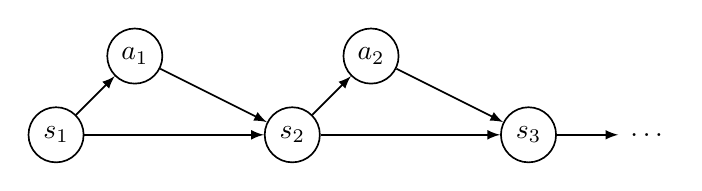
\begin{tikzpicture}[-latex ,auto ,node distance =1 cm and 1cm ,
      on grid , inner sep=0pt, minimum size=7mm,
      semithick, state/.style={circle, draw}]
      % s1, a1, s2;
      \node[state](s_1) at(0,0) {$s_1$};
      \node[state](a_1) at(1,1) {$a_1$};                                                                                                       
      \path (s_1) edge (a_1);
      \node[state](s_2) at(3,0) {$s_2$};
      \path (s_1) edge (s_2);
      \path (a_1) edge (s_2);
      % s2, a2, s3
      \node[state] (a_2) at(4,1) {$a_2$};
      \path (s_2) edge (a_2);
      \node[state] (s_3) at(6,0){$s_3$};
      \path (s_2) edge (s_3);
      \path (a_2) edge (s_3);
      % dots;
      \node (dots) at(7.5,0) {$\ldots$};
      \path (s_3) edge (dots);
  \end{tikzpicture}
  \caption{\label{fig:MDP} Graph of MDP with Markovian states.}
\end{figure}

As mentioned earlier with the robot example, we can have our agent 
not observe the Markovian state, and instead receive an observation, 
$o_t$, from its sensors. This observation is associated with 
an emission operator $\mathcal{E}$, that defines a (possibly stochastic) 
mapping from the state space, $\mathcal{S}$, to the observation 
space, $\mathcal{O}$. This induces a Partially Observed MDP (POMDP) 
whose graphical model is presented in Figure \ref{fig:POMDP}. The 
POMDP is defined by the tuple ($\mathcal{S}$, $\mathcal{A}$, 
$\mathcal{O}$, $\mathcal{P}$, $\mathcal{E}$, $r(\cdot)$, $\gamma$), 
where $\mathcal{O}$ and $\mathcal{E}$ are the observation space and 
the emission operator respectively and everything else in the tuple 
is the same as for the MDP case. It is important to note that the 
reward function is still dependent on the states, and not the observations 
since it specifies the goal and is external to the agent. Intuitively, 
the environment is oblivious to the sensory limitations of the agent 
and only bases its reward signal on the current configuration/state and 
the action that is selected by the agent.

As we 
can read off of the pgm in figure \ref{fig:POMDP}, we see that given 
$s_t$ and $a_t$, $s_{t+1}$ is still independent of 
$o_{1:t}$, $s_{1:t-1}$ and $a_{1:t-1}$ by D-separation.
The observations, however, are not Markovian in general 
(if states are not observed) since $o_j$ for $j<t$ 
can influence $o_{t+1}$ even if $o_t$ and $a_t$ are known (again by 
D-separation).

\begin{figure}[H]
  \centering
  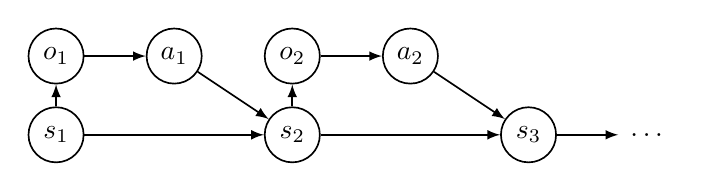
\begin{tikzpicture}[-latex ,auto ,node distance =1 cm and 1cm ,
      on grid , inner sep=0pt, minimum size=7mm,
      semithick, state/.style={circle, draw}]
      % s1, o1, a1, s2;
      \node[state](s_1) at(0,0) {$s_1$};
      \node[state](o_1) at (0, 1){$o_1$};
      \path (s_1) edge (o_1);
      \node[state](a_1) at(1.5,1) {$a_1$};
      \path (o_1) edge (a_1);
      \node[state](s_2) at(3,0) {$s_2$};
      \path (s_1) edge (s_2);
      \path (a_1) edge (s_2);
      % s2, o2, a2, s3
      \node[state](o_2) at (3,1) {$o_2$};
      \path (s_2) edge (o_2);
      \node[state] (a_2) at(4.5,1) {$a_2$};
      \path (o_2) edge (a_2);
      \node[state] (s_3) at(6,0){$s_3$};
      \path (s_2) edge (s_3);
      \path (a_2) edge (s_3);
      % dots;
      \node (dots) at(7.5,0) {$\ldots$};
      \path (s_3) edge (dots);
  \end{tikzpicture}
  \caption{\label{fig:POMDP} Graph of POMDP, $s_t$ is the Markovian 
  state, $o_t$ is the observation of the agent.}
\end{figure}

The associated factorisation based on the pgm in 
figure \ref{fig:POMDP} is:
\begin{equation}
  p^{\pi}(\tau)=p(s_1)\prod_{t=1}^T p(o_t|s_t)\pi(a_t|o_t)p(s_{t+1}|s_t, a_t).
\end{equation}
We see that in the POMDP setting, the agent makes decisions based 
on the observation and not the Markovian state. Depending on how 
informative the observation is, it may be difficult to construct 
a well-performing policy. Additionally, due to the non-Markovian 
nature of the observations, it is common to track and process old 
observations in order to form the agent state. Intuitively, one 
would expect the influence of observations from a long time ago 
to decay, so it might be useful to have a moving window over the 
collected experience.

In cases where we have deterministic transitions from state and action 
to the next state (and similarly from state to observation), 
$p(s_{t+1}|s_t, a_t)=\delta(s_{t+1},f(s_t, a_t))$, where 
$\delta(\cdot)$ denotes the delta distribution (placing all 
probability mass on $f(s_t, a_t)$) and 
$f: \mathcal{S}\times\mathcal{A}\rightarrow \mathcal{S}$ is some deterministic 
transition function (similarly $g:\mathcal{S}\rightarrow \mathcal{O}$ 
can be the sensor mapping the state to the observation).

% SECTION - FORMULATING EPISODIC AND CONTINUAL SETTING REWARD;
\section{Formulating objective functions}\label{sec:RLGoalMaths}
In section \ref{sec:RLGoal} we explained the goal of RL in words. 
In this section we will give a more formal mathematical definition. 
To that end we will first define the finite/episodic case objective, 
and then define the continual setting objective.

First, recall the Monte Carlo return \ref{eq:MCReturn}. The episodic 
objective is to find a behaviour/policy, $\pi(\cdot)$, that maximises 
the expected Monte Carlo return over the distribution of finite 
trajectories, induced by the policy. This is summarised by equation \ref{eq:ep_objective}.
\begin{align}
  \label{eq:ep_objective}
  \pi^*&=\arg \max_{\pi}\; \mathbb{E}_{\tau\sim p^{\pi}(\tau)}[G_0(\tau)]\notag\\
  &=\arg \max_{\pi}\; \mathbb{E}_{\tau\sim p^{\pi}(\tau)}\left[\sum_{t=0}^{len(\tau)}\gamma^tr(a_{t+1}, s_{t+1})\right].
\end{align}
In \ref{eq:ep_objective}, $len(\tau)$ denotes the length of the episode.

Before we tackle the continual setting, observe that the MDP in 
figure \ref{fig:MDP} can be seen as a Markov chain where we define 
the new state $z_t:=(s_t, a_t)$. Based on this formulation we also 
get a new transition operator 
$p(a_{t+1},s_{t+1}|a_t,s_t)=\pi(a_{t+1}|s_{t+1})p(s_{t+1}|a_t,s_t)$ and 
the corresponding pgm can be observed in figure \ref{fig:MCz}.

\begin{figure}[H]
  \centering
  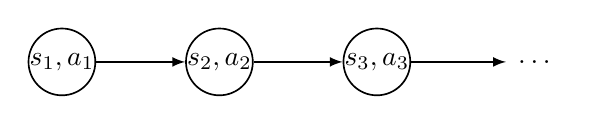
\begin{tikzpicture}[-latex ,auto ,node distance =1 cm and 1cm ,
      on grid , inner sep=0pt, minimum size=7mm,
      semithick, state/.style={circle, draw}]
      % s1, a1, s2;
      \node[state](z_1) at(0,0) {$s_1,a_1$};
      \node[state](z_2) at(2,0) {$s_2, a_2$};
      \path (z_1) edge (z_2);
      \node[state](z_3) at(4,0) {$s_3, a_3$};
      \path (z_2) edge (z_3);
      \node (dots) at(6,0) {$\ldots$};
      \path (z_3) edge (dots);
  \end{tikzpicture}
  \caption{\label{fig:MCz} Markov chain induced by MDP.}
\end{figure}

It can be shown that if the Markov chain is aperiodic and if there 
is a path to all possible tuples $(s_t, a_t)$ from any other tuple 
$(s_j, a_j)$, then an equilibrium distribution exists, which 
tells us the long-term probability of visiting a state-action tuple 
$\mu(s_t, a_t)$.

Observe that we could also rewrite the episodic definition as:
\begin{align}
  \label{eq:cont_objective}
  \pi^*&=\arg \max_{\pi}\; \mathbb{E}_{\tau\sim p^{\pi}(\tau)}[G_0(\tau)]\notag\\
  &=\arg \max_{\pi}\; \mathbb{E}_{\tau\sim p^{\pi}(\tau)}\left[\sum_{t=0}^{len(\tau)}\gamma^tr(a_{t+1}, s_{t+1})\right]\\
  &=\arg \max_{\pi}\; \sum_{t=1}^{maxlen(\tau)}\mathbb{E}_{s_t, a_t\sim p^{\pi}(s_t, a_t)}[r(s_t, a_t)\gamma^{t-1}]\\
  &=\arg \max_{\pi}\; \frac{1}{maxlen(\tau)}\sum_{t=1}^{maxlen(\tau)}\mathbb{E}_{s_t, a_t\sim p^{\pi}(s_t, a_t)}[r(s_t, a_t)\gamma^{t-1}],
\end{align}
where $maxlen(\tau)$ is the maximum length of a trajectory possible under $\pi$. 
In the continual setting, $maxlen(\tau)\rightarrow\infty$, and provided the 
equilibrium distribution for the Markov Chain in \ref{fig:MCz} exists, 
after some time (burn-in), $p^{\pi}\rightarrow \mu^{\pi}$. Additionally,
 due to the division by $maxlen(\tau)$, 
the first finite number of steps from $p^{\pi}$ 
will be negligable and only the steps sampled according to the equilibrium, 
$\mu^{\pi}$ will persist. This intuition, helps us arrive at the 
continual objective known as expected long-term reward:
\begin{equation}\label{eq:continualObjective}
  \arg \max_{\pi}\; {E}_{s, a\sim \mu^{\pi}(s, a)}[r(s, a)],
\end{equation}
where $\mu^{\pi}$ is the limiting distribution of the Markov chain 
induced by $\pi$ \ref{fig:MCz}.



%%%%%%%%%%%%%%%%%%%%%%%%%%%%%%%%%%%%%%%%%%%%%%%%%%%%%%%%%%
% NEW SECTION - VALUE FUNCS;
\section{Value functions}\label{sec:valueFuncs}
A key quantity in our application and of much of modern Reinforcement Learning 
are the value functions. These quantities aim to estimate the 
expected future return, given the current state or state-action pair. 
We shall derive those quantities from the RL objective functions 
defined in the previous section.

Starting from the episodic objective \ref{eq:ep_objective},
\begin{align}\label{eq:valFuncDef}
  \mathbb{E}_{\tau\sim p^{\pi}(\tau)}\left[\sum_{t=1}^{len(\tau)}r(s_t, a_t)\gamma^{t-1}\right]
  &=\mathbb{E}_{s_1\sim p(s_1)}\left[\mathbb{E}_{\tau\sim p^{\pi}(\tau|s_1)}\left[\sum_{t=1}^{len(\tau)}r(s_t, a_t)\gamma^{t-1}|s_1\right]\right]\notag\\
  &=\mathbb{E}_{s_1\sim p(s_1)}\left[
      \mathbb{E}_{a_1\sim \pi(\cdot|s_1)}\left[
          r(s_1, a_1) + 
          \mathbb{E}_{\tau\sim p^{\pi}(\tau|s_1,a_1)}\left[\sum_{t=2}^{len(\tau)}r(s_t, a_t)\gamma^{t-1}\right]|s_1,a_1
        \right]
    \right]\notag\\
  &=:\mathbb{E}_{s_1\sim p(s_1)}\left[
      \mathbb{E}_{a_1\sim \pi(\cdot|s_1)}\left[Q^{\pi}(s_1,a_1)\right]
      \right]\notag\\
      &=:\mathbb{E}_{s_1\sim p(s_1)}\left[
        V^{\pi}(s_1)
      \right],
\end{align}
where $Q^{\pi}(s_1,a_1)$ is the state-action value function,  
sometimes referred to as the Q-function, and $V^{\pi}$ is the state-value 
function.

In \ref{eq:valFuncDef} we already used a form of the Bellman expectation/prediction 
equation:
\begin{align}\label{eq:bellmanv}
  V^{\pi}(s)&=\mathbb{E}_{a\sim \pi(\cdot|s)}[Q^{\pi}(s, a)|s]\notag\\
  &=\mathbb{E}_{a\sim \pi(\cdot|s)}\left[r(s, a) + \gamma \sum_{s'\in \mathcal{S}}p(s'|s,a)V^{\pi}(s')|s\right].
\end{align}

The same for the Q-function is given by equation \ref{eq:bellmanq}.
\begin{align}\label{eq:bellmanq}
  Q^{\pi}(s, a)&=r(s, a) + \gamma \sum_{s'\in \mathcal{S}}p(s'|s, a)V^{\pi}(s')\notag\\
  &= r(s,a) + \gamma \sum_{s'\in \mathcal{S}}p(s'|s, a)\sum_{a'\in \mathcal{A}}\pi(a'|s')Q^{\pi}(s', a').
\end{align}

The other pair of Bellman equations are known as the Bellman optimality 
equations and enforce a consistency criterion for optimal policies. 
\begin{align}\label{eq:bellmanOptV}
  V^{\pi^*}(s)&=\max_{a\in \mathcal{A}}\; \left[r(s, a) + \gamma \sum_{s'\in \mathcal{S}}p(s'|s,a)V^{\pi}(s')|s\right]\notag\\
  &=\max_{a\in \mathcal{A}}\;Q^{\pi^*}(s, a).
\end{align}

\begin{align}\label{eq:bellmanOptQ}
  Q^{\pi^*}(s,a)&=r(s,a) + \gamma \sum_{s'\in \mathcal{S}}p(s'|s, a)\max_{a'\in \mathcal{A}}\;Q^{\pi*}(s', a').
\end{align}

It can be shown that there always exists at least one optimal 
policy \citep{Sutton1998}, and the Bellman optimality equations 
in \ref{eq:bellmanOptV} and \ref{eq:bellmanOptQ} can be viewed 
as consistency equations for an optimal policy $\pi^*$.

% SECTION - improving the policy;
\section{Value iteration}
\textbf{TODO NEED TO FINISH;}
\section{Q-learning}
\begin{itemize}
  \item Mention it's the sampled version of the bellman optimality 
  equation.
  \item Cite the source that proves the convergence.
  \item Mention it's 1-step off-policy method;
\end{itemize}
\section{Policy gradients}
\begin{itemize}
  \item Derive policy grad;
  \item Show that adding a baseline that does not depend on 
  an action, still keeps the update unbiased;
  \item Substitute the baseline for the state-value function 
  and motivate Actor-Critic;
\end{itemize}
\section{Maximum Entropy Reinforcement Learning}\label{sec:MaxEntRL}
\begin{itemize}
  \item Draw pgm based on \citep{LevineRLasInf};
  \item Mention it can also be given as MRF with $\exp(r(s, a))$ 
  as pairwise potential between $s$ and $a$.
  \item Show connection to the Bellman update.
\end{itemize}

%%%%%%%%%%%%%%%%%%%%%%%%%%%%%%%%%%%%%%%%%%%%%%%%%%%%%%%%%%%%%%%%%%
% NEW CHAPTHER - IRL THEORY;
\chapter{Inverse Reinforcement Learning}\label{chap:IRL}
Inverse Reinforcement Learning (IRL) is a method of estimating 
a reward function given expert trajectories/demonstrations 
from performing a given task. Estimating the reward function can be 
useful for learning about how natural systems operate and potentially 
try to mimic their behaviour by learning a policy that 
optimises the 
estimated reward function. Fruthermore, the idea of learning a 
reward function 
is particularly appealing for complex environment settings 
where it is not obvious what the reward function looks like. 
In such settings blindly applying RL to learn a policy may 
prove difficult or infeasible. 


The authors of \cite{NgIRL} 
further argue that in settings where we wish to understand 
the behaviour of a (natural) system, the reward might give an even 
more concise explanation to the observed behaviour 
than learning a policy to mimic the behaviour of the subject 
of study. This statement is based on the assumption 
of RL that any goal can be achieved by maximising a relevant reward 
function.

As shown in \cite{NgIRL}, however, it turns out there are many 
reward functions that explain a given behaviour/policy. Among 
them are degenerate solutions such as reward being zero everywhere, 
and indeed the constant reward function that assigns equal reward 
regardless of the action taken. - \textbf{Not sure if I should give a short proof}

In what follows, we describe ways in which to select ``feasible'' 
reward functions that are not degenerate. 

We cover two such approaches to regularising the reward 
search space. - \textbf{I think I'm fine mentioning the Ng 
approach with SVM heuristic and not go into too much detail 
since I end up using the MaxEnt IRL approach}


The first approach is heuristic-based \citep{NgIRL} and 
aims to find 
a reward function according to which the observed expert behaviour 
is maximally optimal/different relative to any other behaviour. The 
authors of \cite{NgIRL} formulate this problem as a linear problem, 
very similar to the problem setting of Support Vector Machines 
(SVMs) \citep{SVMs}, where the goal is to find a hyperplane that 
best separates the expert behaviour/policy from any other policy. 
In the continuous state space setting, the reward in \cite{NgIRL} 
is linear in its parameters who have similar constraints to 
the hyperplane in SVMs.

\textbf{TODO: GIVE THE MATHS}
The second approach, is the Maximum-Entropy IRL approach 
\citep{Ziebart2008}, that aims to find a reward that induces 
a policy who apart from matching the features of 
states along the paths of the expert demonstrations (feature 
matching), has 
to act as randomly as possible (maximum entropy). To do this, 
\cite{Ziebart2008} effectively do maximum likelihood learning 
for the parameters of the reward function in the setting of 
Maximum Entropy RL \ref{sec:MaxEntRL}. Due to using a linear 
function approximation for the reward in \cite{Ziebart2008}, 
we get a familiar equation for parameter estimation, reducing 
to matching expected sufficient statistics of an exponential 
family distribution over trajectories. 


% \begin{itemize}
  % \item model known and complete policy is given;
  % \begin{itemize}
    % \item discrete state space - linear programming;
    % \item continuous state space - linear func approx;
  % \end{itemize}
  % \item many rewards possible based on policy (ill posedness);
  % \begin{itemize}
    % \item use svm heuristic - solve with linear prog in discrete state case;
    % \item for cont cases again solvable by linear progs;
  % \end{itemize}
  % \item if expert policy only trough finite num of traj, 
  % solve with iterative algo;
% \end{itemize}

\begin{itemize}
  \item State the goal of IRL - estimate an objective function
    that when optimised should yield a behaviour similar to the 
    one in the demos by the expert.
  \item Argue the point about the ill-posedness of IRL, which makes 
    classic optimal control not suitable for the job.
  \item Talk about the max-margin approach (Ng) to IRL.
    State drawbacks;
  \item Give the update equation for the rewards in the 
  continuous state space setting - rewards on expert traj 
  vs rewards with imp-weights due to sampling;
\end{itemize}

%%%%%%%%%%%%%%%%%%%%%%%%%%%%%%%%%%%%%%%%%%%%%%%%%%%%%%%%%%%%%%%%%%
% NEW CHAPTER - GRAPH REPRESENTATIONS;
\chapter{Graph representations}\label{chap:GNNs}
\begin{itemize}
  \item the current stuff might be a bit verbose and talks 
  a bit too much about general DL; 
  \item I am thinking, just start directly with \cite{ScarselliGNN};
  \item Mention a few prominent works such as \cite{MPNNs,GCN};
  \item Give the relevant equations for a general neural message 
  passing procedure;
  \item finish off with the GATv2 \citep{GATv2} architecture, 
  since this is what I am using.
  \item Give the equations for GATv2 and connect it to the 
  attention mechanism \citep{transformers}.
  \item State drawbacks and potential reasons, why it is difficult 
    to work with graph topography rather than topology when using 
    GNNs - perm inv agg over nodes loses info.
\end{itemize}
Currently, Deep Learning (DL) is among the most prominent paradigms 
for representation learning. Although the advent of the 
Multilayered Perceptron (MLP) dates back to 
1958 \citep{perceptron}, DL saw a long period 
of stagnation. After the successful application of 
Convolutional Neural 
Networks (CNNs) \citep{CNNsLecun} to image classification
in the ImageNet challenge 
\citep{alexnet,imagenet}, however, DL regained 
its popularity. The unprecedented success 
popularised DL as a prominent way 
to obtain expressive representations of abstract data types. 
Apart from image classification, 
Deep Learning has also been successfully 
applied to text domains in problems such as 
sentiment analysis \citep{SentimentRNN,textCNN,BERT},  
natural language translation \citep{nlpTranslation},
and generative autoregressive systems \citep{GPT,GPT2020}.

Efficient implementations \citep{PyTorch,tensorflow} 
of the Backpropagation algorithm \citep{backprop} and the 
advance of computing 
hardware have also encouraged the development of highly parallelisable 
model classes such as the Transformer \citep{transformers}. The 
Transformer currently plays a key role in achieving the 
State-Of-The-Art (SOTA) performance 
in various fields and efforts are made to adopt the attention 
mechanism to other areas.

Theoretical work \citep{UnivApproxNN} has also established
that under some conditions, sufficiently deep MLPs 
can be used as universal function approximators. To this end, 
MLPs have also been used to map random noise from a latent 
dimension to the data dimension, approximating 
the data generating process \citep{goodfellow2014generative,VAEs}.

An area that is particularly relevant for this work, 
is Deep Reinforcement Learning 
(DRL). In their application, \cite{DQN}, use a CNN directly on 
raw image pixels to approximate the Q-function, part of a 
Q-learning algorithm \citep{QlearningWatkins1992}. 

In contrast to images, that can be thought of as grid-like graphs 
(where each pixel/node is connected to the neighbouring pixels), 
general graphs are difficult to represent using standard 
neural architectures such as MLPs. While one can use an MLP 
to learn embeddings of the nodes of a graph, this does not 
account for the connectivity of the graph, specified by the edge set. 
These limitations of standard Deep Neural architectures 
have motivated the invention of Graph Neural Networks (GNN) \citep{ScarselliGNN}. 
These models have found applications in areas such as 
Quantum Chemistry \citep{MPNNs}, where 
a general form of the Message Passing Neural Net (MPNN) was 
introduced.



%%%%%%%%%%%%%%%%%%%%%%%%%%%%%%%%%%%%%%%%%%%%%%%%%%%%%%%%%%%%%%%%%%
% NEW CHAPTER - OUR CONTRIBUTION;
\chapter{The baseline model and our contribution}\label{chap:contribution}
% In practice, learning a graph generative mechanism is challenging 
% since, most of the time, we are not provided with (multiple) demonstrations 
% of the graph building process. Instead, we are only given the 
% final constructed graph.
\begin{itemize}
  \item Describe GraphOpt;
  \item Describe our spin on it:
  \begin{itemize}
    \item Separate reward func encoder;
    \item Per-dec imp samples;
    \item UT trick if results are good;
  \end{itemize}
  \item Maybe also give some notes on technical 
  implementation for efficiency with the replay buffer 
  where we only save state-action data and eval rewards 
  at batch sampling time; that way we don't have to clear the 
  buffer after reward update every time;
\end{itemize}

%%%%%%%%%%%%%%%%%%%%%%%%%%%%%%%%%%%%%%%%%%%%%%%%%%%%%%%%%%%%%%%%%%
% NEW CHAPTER - EXPERIMENTS;
\chapter{Experiments}\label{chap:experiments}

\section{Description of tests}
\label{sec:test_description}
The experimental suite consists of four tests.
\begin{algorithm}
  \caption{Reward function transfer vs direct policy deployment}
  \label{tests:test_reward_transfer}
  \begin{algorithmic}
    \State $irlreward,\; irlpolicy \gets irlalgorithm(sourcegraph)$
    \State $irlstats,\; newpolicystats \gets [],\; []$
    \For{$t=1\ldots k$}
    \State $irlstats_t \gets collect\_irlstats(targetgraph)$
    \State $newpolicy_t \gets train\_policy(targetgraph,\; irlreward)$
    \State $newpolicystats_t \gets collect\_newpolicystats(targetgraph)$
    \State $irlstats.append(irlstats_t)$
    \State $newpolicystats.append(newpolicystats_t)$
    \EndFor
    \State $return\; (irlstats,\; newpolicystats)$
  \end{algorithmic}
\end{algorithm}
In Algorithm \ref{tests:test_reward_transfer}, by ``stats'', it is meant 
graph topology statistics such as triangles, clustering coefficients, 
degrees and rewards along generated paths associated with the 
relevant policy. The \verb|collect_stats| function deploys the relevant 
policy on the vertex set of the relevant graph (starting with an 
empty edge set). The termination condition is when we have build the same 
number of edges as the original graph (passed to the \verb|collect_paths|
function) or when along the process of graph building we propose 
too many repeated edges (edges we had added earlier) or 
self-loops (connects a node to itself).

After these numbers are saved, we calculate summary 
statistics such as \verb|min|, \verb|median|, \verb|max|, 
\verb|mean|, \verb|standard_deviation| and 
then report the average and the standard deviations of the five number 
summaries ($k$ total) over the $k$ runs. For example, for each of the 
$k$ passes of the for loop of algorithm \ref{tests:test_reward_transfer} 
we get the degrees of all nodes, then take the \verb|median| degree for 
that pass and append it to the medians of the other passes. This way 
we obtain the median degree for each of the $k$ passes. We then average 
the $k$ numbers and calculate the standard deviation. The final reported 
value will then be the average median degree over $k$ passes, together 
with its standard deviation.

Based on the raw graph topology statistics (e.g., we concatenate the 
degrees of the nodes over the $k$ passes), we report the 
p-values from a two-sample Kolmogorov-Smirnov (KS) \citep{KSTest} 
test against the 
graph topology statistics of the true graphs (source or target graph). 
This way we usually compare the distribution of a sample of $k\times |\mathcal{V}|$ 
numbers versus the distribution of $|\mathcal{V}|$ numbers (the latter being the 
true graph statistics), where $|\mathcal{V}|$ denotes the number 
of nodes/vertices in the relevant graph.

This test is used to determine whether we were able to learn a better 
graph construction policy for the target graph 
by retraining a new policy using the IRL-reward 
or by directly deploying the IRL-policy on the target graph.

Since the irlpolicy was trained on the source graph, we should expect 
it to construct a graph on the targetgraph's vertex set, that resembles 
the topology of the source graph. On the other hand, if the source 
graph and the target graph are very similar, we should expect 
the learned reward from IRL (on the source graph) to give a useful 
criterion to guide the 
newpolicy in constructing graphs with similar topology to that 
of the target graph.

\begin{algorithm}
  \caption{Learning the source graph distribution}
  \label{tests:test_learn_source_graph_dist}
  \begin{algorithmic}
    \State $irlreward,\; irlpolicy \gets irlalgorithm(sourcegraph)$
    \State $irlstats \gets []$
    \For{$t=1\ldots k$}
    \State $irlstats_t\gets collect\_irlstats(sourcegraph)$
    \State $irlstats.append(irlstats_t)$
    \EndFor
    \State $return\; irlstats$
  \end{algorithmic}
\end{algorithm}
The second test we employ, is used to determine if the trained 
irlpolicy can be used 
to build graphs similar to the source graph (in terms of topology). 
The pseudocode for this test is provided in Algorithm 
\ref{tests:test_learn_source_graph_dist}.
As in the previous test, the \verb|collect_irlstats| 
function deploys 
the policy on the vertex set, having emptied the edge set.

Similarly to Algorithm \ref{tests:test_reward_transfer}, ``stats'' 
refers to the graph topology statistics described above. We again 
calculate averages and standard deviations of the summary statistics 
over the $k$ runs, as well as p-values from the KS test.

Since the irlpolicy was trained on the source graph during IRL, 
we should expect it to be able to reconstruct graphs with similar 
topological properties. We judge how well the irlpolicy constructs 
graphs that are topologically similar to the source graph 
based on the p-values 
from two-sample KS tests.

\begin{algorithm}
  \caption{Held-out edges prediction}
  \label{tests:test_edge_prediction}
  \begin{algorithmic}
    \State $train\_edges,\; val\_edges \gets split(sourcegraph,\; proportion)$
    \State $irlreward,\; irlpolicy \gets irlalgorithm(sourcegraph)$
    \State $mrrs,\; prop\_guessed \gets [],\;[]$
    \For{$t=1\ldots k$}
      \State $ranks,\; flag \gets [],\; True$
      \State $guesses\_dict=\{e:\; 0\; for\; e\; in\; val\_edges\}$
      \State $s \gets env.start\_from\_train\_edges()$
      \While{episode not finished}
        \State $ps \gets irlpolicy(s, k\_proposals)$
        \State $action\gets ps[0]$
        \State $position=\infty$
        \For{$i,\; a\; in\; enumerate(ps,\; start=1)$}
          \If{$a$ is repeated or is self loop}
            \State continue
          \EndIf
          \If{$flag$}
            \State{$action\gets a$}
            \State{$flag\gets False$}
          \EndIf
          \If{$a\in val\_edges$}
            \State $position=i$
            \State $guesses\_dict[a] = 1$
            \State $break$
          \EndIf
        \EndFor
        \State{$ranks.append(1/position)$}
        \State{$s\gets env(action)$}
      \EndWhile
      \State{$mrrs.append(mean(rank))$}
      \State{$prop\_guessed.append(sum(guesses\_dict.values())/len(val\_edges))$}
    \EndFor
    \State{$return\; summary(mrrs),\; summary(prop\_guessed)$}
  \end{algorithmic}
\end{algorithm}

The third test evaluates the learned irlpolicy on a task it was not 
explicitly trained on - missing edge prediction. We judge how good 
the irlpolicy is at predicting the missing edges by reporting summary 
statistics of Mean Reciprocal Ranks (MRR) and proportions of held-out 
edges that were guessed during the course of graph construction.
These summaries are done over $k$ runs 
of graph constructions starting with the vertex set of the source 
graph, and edge set initialised with the edges that were 
available for training (treated as expert demos wrt IRL). 

The MRR tells us the ``preference'' 
of the policy for the held-out edges. As can be seen in Algorithm 
\ref{tests:test_edge_prediction}, each rank is in the range $[0, 1]$. 
If a held-out edge is at the $n^{th}$ position in the list of proposals 
$ps$, then its reciprocal rank for that iteration is $1/n$. Alternatively, 
if none of the proposed actions in $ps$ are in the held-out edge set, 
the reciprocal rank is $1/\infty\rightarrow 0$. This shows, that the 
best possible MRR score is $1$, corresponding to a held-out edge 
always being the first proposed action in the list of proposals $ps$.

The proportion of guessed edges tells us what proportion of the 
hel-out edges were proposed during the graph construction process. 
The python dictionary implementation in Algorithm \ref{tests:test_edge_prediction} 
prevents double-counting edges if they are proposed multiple times.

\begin{enumerate}
  \item Experimental Recipe:
  \item Run IRL training on a source graph. Receive trained policy 
  and reward function.
\end{enumerate}
\begin{itemize}
  \item T1 is about transferring learned reward on target graph;
  also compares learned policy directly on target, compared to 
  training new policy on target with frozen reward;
  \item T2 is about MRR - based on top 25 proposal edges;;
  \item T3 is about running learned policy on source graph and 
  seeing if we get similar graphs;
  \item I also get rewards along paths.
  \begin{itemize}
    \item Compare convergence rate of eval returns over seeds
      and comment on speed;
  \end{itemize}
  \item BA40 to BA80 - 10 seeds
  \begin{itemize}
    \item GOptEpWeights, GOptPerDec, 
      GOptRewEncEpWeights, GOptRewEncPerDec,
    \item THIS IS NOT APPLICABLE TO BA GRAPHS - ONLY TRY IT ON GRAPHS 
      WITH MEANINGFUL TOPOGRAPHY!!! - Then take better of EpWeights and PerDec and do 
      GOptMultitaskBetterWeight and GOptRewEncMultitaskBetterWeight,
    \item also run UT trick with the better weight setting;
  \end{itemize}
    
  \item T1 and T3 run together - this is $10\times 8=80$ experiments;
  \item T2 runs alone - this is $10\times 8=80$ experiments;
  \item total is 160 experiments;
  \item  Run best config on Urban nets 10 times;
\end{itemize}

\chapter{Conclusion and Further work}\label{chap:conclusion}
This work builds on prior research in inverse reinforcement learning 
for graph domains. Our contributions are, firstly, the addition of the 
per-decision importance sampling for the IRL reward objective, 
secondly, the addition of a graph encoder to the reward function, 
and finally, an empirical comparison of applying the Unscented 
Transform \citep{JulierUT} versus the reparameterisation trick 
for approximating expectations.

We have empirically shown that the per-decision importance 
sampling increases
the stability of the algorithm over multiple seeds as seen by 
the plots of the returns during training.

Adding a graph encoder as part of the reward function, seems to 
have helped learn appropriate embeddings, which were useful for 
evaluating the states on the target graph. This is seen in the 
performance comparison between this method and 
the vanilla GraphOpt \citep{GraphOpt} 
implementation which uses a single graph encoder. Our method 
also allows for the ``full'' transfer of the reward function, 
rather than simply taking the MLP associated with the reward and 
then retraining a graph encoder and a policy. The latter actually 
can ``trick'' the reward to think a state is more advantageous than 
it actually is by providing an ``adversarial'' embedding that is 
mapped to a high reward from the reward MLP. Providing the reward 
with its own graph encoder, helped avoid such situations.

Finally, we showed that the UT trick also lead to more stable 
training of the algorithm as seen by the plots of the losses 
and the returns recorded during evaluation.

Despite the proposed improvements, it is still unclear what constitutes 
a good strategy for generating expert samples for the IRL objective. 
Merely giving a random permutation of the edge set removes the possible 
temporal component in building the graph. In many cases, such as 
road-network planning, previously built connections can actually 
be the main reason for new road segments. As a simple illustration 
of this idea, the reader is directed to Figure \ref{fig:bad_rand_perm}.
In contrast to most IRL scenarios where new demonstrations are generated, 
we only work with a single demonstration, which we assume the temporal 
component has no effect, allowing us to treat any permutation of the 
edge set as a separate expert trajectory. As seen in the figure, this 
could lead to very different demonstrations from the optimal control 
demonstration and may result in learning poor policies.

\begin{figure}[H]
  \centering
  \includegraphics[scale=0.5]{bad_rand_perm.png}
  \caption{\label{fig:bad_rand_perm} Optimal control path 
  in blue colour for both plots. The ``optimal control path'' 
  is simply a $sin(\cdot)$ function. The two x-marks are the 
  starting and ending point of all paths. It is assumed 
  we always start from the same position and the ``goal'' is also 
  at the same position. Left: different soft-optimal 
  paths sampled alongside the optimal control path (soft-optimal 
  paths generated by adding random Gaussian noise to the optimal 
  path). Right: different 
  random permutations of the optimal control path sampled alongside 
  the optimal control path.}
\end{figure}


% \chapter{title of first chapter}
% This is just a bare minimum to get started.  There is unlimited guidance on using latex, e.g. {\tt https://en.wikibooks.org/wiki/LaTeX}.   You are still responsible to check the detailed requirements of a project, including formatting instructions, see \\
% {\tt https://moodle.ucl.ac.uk/pluginfile.php/3591429/mod\_resource/content/7/UGProjects2017.pdf}.
% Leave at least a line of white space when you want to start a new paragraph.

% Mathematical expressions are placed inline between dollar signs, e.g. $\sqrt 2, \sum_{i=0}^nf(i)$, or in display mode
% \[ e^{i\pi}=-1\] and another way, this time with labels,
% \begin{align}
% \label{line1} A=B\wedge B=C&\rightarrow A=C\\
% &\rightarrow C=A\\
% \intertext{note that}
% n!&=\prod_{1\leq i\leq n}i \\
% \int_{x=1}^y \frac 1 x \mathrm{d}x&=\log y
% \end{align}
% We can refer to labels like this \eqref{line1}.   

% \chapter{title of second chapter}
% % Often lots of citations here (and elsewhere), e.g. \cite{Rey:D} or \cite[Theorem 2.3]{PriorNOP70}.   Bibtex can help with this, but is not essential. If you want pictures, try

% \begin{center}
% \includegraphics[scale=.5]{aristotle.jpg}
% \end{center}
% You can use 
% \begin{itemize}
% \item lists
% \item like this
% \end{itemize}
% or numbered
% \begin{enumerate}
% \item like this,
% \item or this
% \end{enumerate}
% but don't overdo it.
% \chapter{title of third chapter}
% If you have a formal theorem you might try this.
% \begin{definition}\label{def}
% See definition~\ref{def}.
% \end{definition}
% \begin{theorem}
% For all $n\in\nats,\; 1^n=1$.
% \end{theorem}
% \begin{proof}
% By induction over $n$.
% \end{proof}

% \chapter{etc.}
\appendix

\bibliographystyle{apa}
\bibliography{my_bib.bib}

\end{document}